%This is the second chapter of the dissertation

%The following command starts your chapter. If you want different titles used in your ToC and at the top of the page throughout the chapter, you can specify those values here. Since Columbia doesn't want extra information in the headers and footers, the "Top of Page Title" value won't actually appear.

\pagestyle{cu}
\graphicspath{{./Chapter2/Figures/}}
\chapter[Liquid Xenon and Time Projection Chambers][Liquid Xenon and Time Projection Chambers]{Liquid Xenon and Time Projection Chambers}
\label{chap:liquid_xe}

Liquid xenon (LXe) direct detection experiments have dominated the sensitivity for WIMP masses $\gtrsim 20$ for approximately as
decade.  Even over liquid argon (LAr) the LXe results have been paved the way to new limits, surpassing on the way only those of other
LXe experiments.

Commercial business, such as steelmaking and coal gasification, rely relatively pure oxygen or nitrogen.  During the separation,
the small amount of xenon and krypton in the air is extracted into a mixture as a by-product.  A distillation process can uncouple
the two, leaving highly pure xenon.

%====================================
\section{General Properties}
\label{sec:properties}
Xenon has an atomic number of 54 with a mean mass of 131.293 g mol$^{-1}$.  Because it is a noble gas it does not easily undergo chemical
reactions with other elements.  It makes up 87 parts per billion (ppb) of the Earth's atmosphere at a density of
5.894 g L$^{-1}$.  \tabref{tab:xe_properties} gives some general chemical properties for xenon.

Xenon is the heaviest noble gas that is non-radioactive, with an atomic molar mass of $A = 131.293\ \mathrm{g\ mol^{-1}}$.  The naturally
occurring Xe isotopes are listed in
\tabref{tab:xe_isotopes}.  $^{136}Xe$, with a fractional percentage of 8.8573\%,
has been measured to undergo double beta decay with a half-life of $> 2.4 \times 10^{21}\ \mathrm{yrs}$ via
$2\nu \beta^{-} \beta^{-}$.  So while technically naturally occurring xenon is radioactive, the process is extremely rare.

Primary and secondary scintillation, which are the measured parameters in a time-projection chamber, occur when a particle interacts
with a Xe atom.  In the case of a neutron or neutrino scattering from the Xe nucleus a number of nuclear excitations are possible,
and are listed in \tabref{tab:xe_radioactive}.  The 39.6 and 80.2 keV lines from $^{129}$Xe and $^{131}$Xe are short-lived and typically cannot
be resolved from the scintillation of the scatter.  However, the 163.9 and 236.14 keV lines from $^{131\mathrm{m}}$Xe and
$^{129\mathrm{m}}$Xe are long-lived
enough to become uniformly distributed throughout the detector and can be used as a calibration source and measuring the electron
lifetime (\chapref{chap:purity}).

Xenon has several advantages that make it a good source for DM detection.  At \$2000 it is scaleable for larger detectors.  Its
large molar mass provides strong self-shielding, which reduces contamination in the region of interest due to external radiation
(discussed in \secref{}).  Furthermore, nearly 50\% of naturally occurring xenon is $^{129}$Xe or $^{131}$Xe, which gives it sensitivity to
spin-dependent interactions.  Its light and charge yields (\secref{}) are the highest among noble gases.  Finally, the amount of
intrinsic radioactivity comes only from 

 
\begin{table}[t]
 \centering
 \begin{tabular}{cc}
 \hline
 Chemical Property & Value \\
 \hline
 Atomic Number & 54 \\
 Molar mass & 131.293 g mol$^{-1}$ \\
 Melting point (1 atm) & -111.75 $^{\circ}$C \\
 Boiling point (1 atm) & -108.099 $^{\circ}$C \\
 Density as gas (0 $^{\circ}$C, 1 atm)  &  5.894 g L$^{-1}$ \\
 Density as liquid (-108.099 $^{\circ}$C, 1 atm) & 2.942 g cm$^{-3}$ \\
 Critical point & 16.59 $^{\circ}$C, 57.65 atm, 1.155 g cm$^{-3}$ \\
 Dielectric constant (liquid) & 1.95 \\
 Triple point & -111.74 $^{\circ}$C, 0.805 atm, 3.08 g cm$^{-3}$ \\
 Thermal conductivity & $5.65 \times 10^{-3}\ \mathrm{W\ m^{-1}\ K^{-1}}$ \\
 Covalent radius & $140 \pm 9$ pm \\
 \hline
 \end{tabular}
 \caption{Chemical properties for Xe}
\label{tab:xe_properties}
\end{table}[t]


\begin{table}
 \centering
 \begin{tabular}{ccccc}
 \hline
 Isotope & Natural Abundance [\%] & Spin & Half-life & Decay mode \\
 \hline
 $^{124}$Xe & 0.0952 & 0 &  $> 1.6 \times 10^{14}\ \mathrm{yrs}$ & $2\nu \beta^{+} \beta^{+}$ \\
 $^{126}$Xe & 0.0890 & 0 & $> 4.7-12 \times 10^{25}\ \mathrm{yrs}$ & $2\nu \beta^{-} \beta^{-}$ \\
 $^{128}$v & 1.9102 & 0 & stable & - \\
 $^{129}$Xe & 26.4006 & 1/2 & stable & - \\
 $^{130}$Xe & 4.0710 & 0 & stable & - \\
 $^{131}$Xe & 21.232 & 3/2 & stable & - \\
 $^{132}$Xe & 26.9086 & 0 & stable & - \\
 $^{134}$Xe & 10.4357 & 0 &  $> 5.8 \times 10^{22}\ \mathrm{yrs}$ & $2\nu \beta^{-} \beta^{-}$ \\
 $^{136}$Xe & 8.8573 & 0 &  $> 2.4 \times 10^{21}\ \mathrm{yrs}$ & $2\nu \beta^{-} \beta^{-}$ \\
 \hline
 \end{tabular}
 \caption{Properties of naturally occurring Xe isotopes.  Decays of $^{124}Xe$, $^{126}Xe$, and $^{134}Xe$ have not been observed
 but are predicted.  Half-life and decay information is taken from \citeref{Singh2007, Barros2014}.}
\label{tab:xe_isotoes}
\end{table}


\begin{table}
 \centering
 \begin{tabular}{ccc}
 \hline
 Isotope & Energy & Half-life \\
 \hline
 $^{129}$Xe & 39.6 keV 0.97 ns & \\
 $^{129\mathrm{m}}$Xe & 236.14 keV & 8.88 d \\
 $^{131}$Xe & 80.2 keV & 0.48 ns \\
 $^{131\mathrm{m}}$Xe & 163.9 keV & 11.93 d \\
 \hline
 \end{tabular}
 \caption{Nuclear excited states for naturally occurring xenon in the energy range direct DM searches are sensitive too.}
 \label{tab:xe_radioactive}
\end{table}


A charged particle passing through a medium will lose energy through inelastic collisions with electrons, prompting ionization or excited
states.  The energy lost per unit
length is the electronic stopping power and denoted $dE/dx$, which is related to the linear energy transfer (LET).  It depends on the
type and energy of the particle and properties of the
medium including density and composition.  A larger electronic stopping power indicates the particle will slow more quickly, thereby
depositing its energy densely along its trajectory.  This is known as self-shielding, and is an
important characteristic of a detector.  A larger self-shielding will restrain external radiation from penetrating deep in the detector,
which allows a larger fiducial volume (FV) for dark matter detection.  Because the stopping power is proportional to the
density of the medium, LXe is more effective at self-shielding than liquid argon ($1.395\ \mathrm{g\ cm^{-3}}$) and liquid neon
($1.207\ \mathrm{g\ cm^{-3}}$).

By dividing the stopping power by the medium's density we get a function that is mainly a function of the radiating particle known as
the mass stopping power.  This is shown for $\alpha$, $e^{-}$, and protons in \figref{fig:mass_stopping_power}.  We see that for the DM
region of interest ($1--100$ keV) as \electron
energy increases the stopping power decreases, while for \alpha and protons the reverse is true.  Multiplying by the density of LXe
$\rho_{\mathrm{LXe}}$ gives an electron stopping power of $0.65--30$ keV/$\mathrm{\mu m}$ for \electron and $\sim 20--900$
keV$\mathrm{\mu m}$ for \alpha and protons.

We can see that in
the dark matter search region ($1-100$ keV) $e^{-}$ decrease by a factor of $\sim 10$.  Multiplying by the density of LXe we get the
electronic stopping power to be $\sim 0.65--30\ \mathrm{keV/\mu m}$.  $\alpha$ decays are typically $> 5.5$ MeV and thus have a stopping
power of $\sim 600--2000\ \mathrm{keV/\mu m}$.  We see that particle tracks are on the order of $10 \mathrm{\mu m}$, so particles that
originate at or outside the surface of the detector will never make it into the FV with any reasonable probability.

\begin{figure}[t]
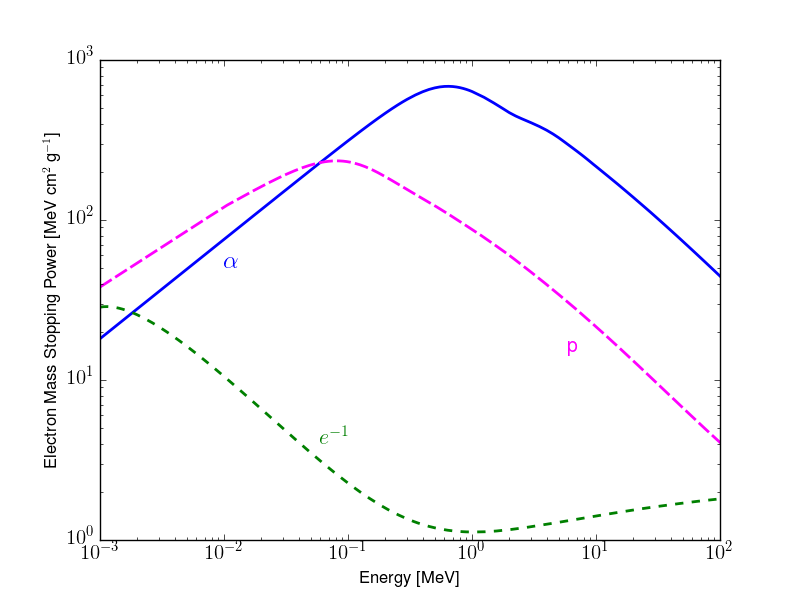
\includegraphics[width=0.8\textwidth]{MassStoppingPower}
\caption{Electron mass stopping power for $\alpha$, $e^{-}$, and protons.  (\citeref{Berger2018a})}
\label{fig:mass_stopping_power}
\end{figure}[t]

Since a higher stopping power translates to a larger decrease in energy, there will be a higher ionization density in the particle
track.  This has implications that will be discussed in \secref{}.



%====================================
\section{Primary and Secondary Scintillation}
\label{sec:scintillation}
Radiation scattering off a xenon atom will produce a prompt or primary scintillation as a result of electronic excitation or recombination
from ionized electrons that emit photons as they de-excite.  Secondary scintillation results from ionized
electrons that do not recombine and is measured only in a time-projection
chamber (TPC).  In this section
and the remainder of the chapter I will consider interactions in xenon in the presence of an electric field, unless otherwise
specified.

When a particle scatters off a Xe atom it can excited or ionize its valence electrons.  Here we refer to excited atoms Xe$^{*}$ as
excitons.  An ionized electron can then escape or recombine with the Xe$^{+1}$.  Excitons can form with another Xe atom to create
dimers, Xe$_{2}^{*}$, commonly referred to as excimers.  The processes recombination is shown in \eqnref{eq:recomb}, where $Q$
represents heat.  It should be stated that the $e^{-}$ in the recombination process is from the same or another ionized atom.  If
no electric field is , so the primary scintillation will not reflect the true

If
an electric field is applied some $e^{-}$ will be forced away from the interaction, thereby lowering recombination and the primary
scintillation.  This effect depends on the strength of the electric field.  However, even if no field is applied there will not be
100\% recombination as some of the freed $e^{-}$ will escape the electromagnetic pull.

\begin{equation}
\mathrm{Xe}^{+} + \mathrm{Xe} \rightarrow \mathrm{Xe}_{2}^{+} \\
\mathrm{Xe}_{2}^{+} + e^{-} \rightarrow \mathrm{Xe}^{**} + \mathrm{Xe} \\
\mathrm{Xe}^{**} \rightarrow \mathrm{Xe}^{*} + Q \\
\label{eq:recomb}
\end{equation}

\noindent At this point the Xe$^{*}$ that has been born of the ionization and recombination process is equivalent to one from simply the
excitation.  At this point they must de-excited via \eqref{eq:deexcite}.  Xe$_{2}^{*}$ is in either a singlet
($^{1}\Sigma$) or triplet ($^{3}\Sigma$) state, and de-excites to the ground state.

\begin{equation}
\mathrm{Xe}^{*} + \mathrm{Xe} \rightarrow \mathrm{Xe}_{2}^{*} \\
\mathrm{Xe}_{2}^{*} \rightarrow 2\mathrm{Xe} + \gamma
\label{eq:deexcite}
\end{equation}

\noindent $\gamma$ is the average de-excitation energy that carries a wavelength of 178 nm.  The lifetimes for the singlet and triplet
excimers are $3.1 \pm 0.7$ ns and $24 \pm 1$ ns, respectively (\citeref{Mock2014}).  The single-to-triplet ratios for
various interaction types are shown in \tabref{tab:singlet_to_triplet}.  An important method for detecting WIMPS is ER-NR
discrimination, and we see that NR recoils result in a substantially higher fraction of singlet states.  Unfortunately the lifetimes
are too short to resolve in a TPC to be able to use for discrimination.  This makes single-phase LXe detectors
less desirable than liquid argon (LAr), which has single and triplet states of $< 6.2$ ns and $1.30 \pm 0.06\ \mathrm{\mu s}$
(\citeref{Heindl2011}).

\begin{table}[t]
 \centering
 \begin{tabular}{cc}
 \hline
 Event & Single/Triplet Ratio \\
 \hline
 ER (direct excitation from $\gamma$) & $0.17 \pm 0.05$ \\
 ER (recombination from $\gamma$) & $0.8 \pm 0.2$ \\
 ER (from $\alpha$) & $2.3 \pm 0.51$ \\
 NR (from neutron) & $7.8 \pm 1.5$ \\
 \hline
 \end{tabular}
 \caption{Error-weighted average of world data for single/triplet ratio for various scattering cases (\citeref{Mock2014}).}
\label{tab:singlet_to_triplet}
\end{table}[t]


\eqnref{eq:recomb} and \eqnref{eq:deexcite}
depict the entire microphysical processes for $\beta$ and $\gamma$ interactions (\citeref{Hitachi2005}).  However, in high linear
energy transfer (LET) with $\alpha$ or fission fragments it has been observed that two excitons may collide and free an electron as
shown in \eqnref{eq:biexitonic}.

\begin{equation}
\mathrm{Xe}^{*} + \mathrm{Xe}^{*} \rightarrow \mathrm{Xe} + \mathrm{Xe}^{+} + e^{-}
\label{eq:biexitonic}
\end{equation}

\noindent This effect is known as biexcitonic quenching and is expected to be the result of excitons being close enough to
interact.  In \beta and \gamma interactions the energy track is sufficiently sparse such that the chances of two excitons doing so
is close to 0.  However, for particles that have a large electron stopping power - such as \alpha or fission fragments - the
density of energized atoms is enough to provoke this.  Biexcitonic quenching signifies the reduction of observed signal, as what would
have been two emitted photons is instead a single \electron with energy close to that of an exciton.

Interactions inside a LXe will free \electron with various energies.  The Onsager radius is defined to be the radius between parent
ion and \electron where the Coulomb energy equals the \electron thermal energy (\citeref{Onsager1938}).  An \electron within this
radius will be unlikely to
escape so will recombine with its parent (the probability of escape at the Onsager radius is $e^{-1}$).  On the contrary, an \electron
with $E_{thermal} > E_{Coulomb}$ will escape - even without the presence of an Electric field.  This results in a decrease of expected
photons.  It is expected in the absence of a field recombination may occur on timescales $> 1$ ms but this is much larger than the
observation window.  The thermalization range for LXe is $4000--5000$ nm, far higher than the Onsager radius of $49$ nm
\citeref{Doke2002}.  If an electric field is applied the \electron that have sufficiently large thermal energy are drifted for
proportional scintillation, conserving the measurable quantity.

The decrease in scintillation yield for \beta and \gamma is only observed at low LET where the ionization density is relatively low.  The
lack of neighboring $\mathrm{Xe}^{+}$ limits the probability of recombination with a non-parent ion.  At higher LET the ion density
is sufficient for essentially 100\% recombination and results in a flat top region as seen in \figref{fig:scintillation_yield}.  This
effect is not technically quenching because there is no true decrease in photons and electrons.

\begin{figure}
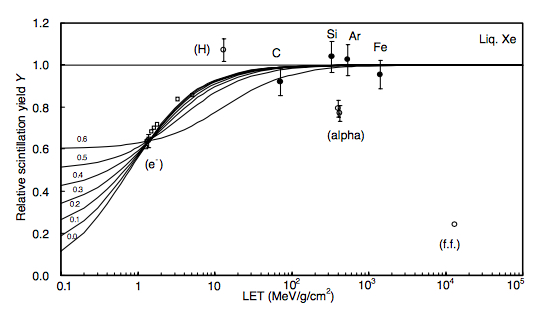
\includegraphics[width=0.8\textwidth]{ScintillationYield}
\caption{Scintillation yield as a function of LET in LXe.  Open circle represent electrons, alpha particles, and fission fragments.  Solid
circles represent relativistic heavy particles.  Open squares represent gamma-ray.  Solid lines represent various fits to the \beta-\gamma
data performed in \citeref{Doke2002} and are not discussed here.  Image credit: \citeref{Doke2002}.}
\label{fig:scintillation_yield}
\end{figure}

Another source of quenching besides biexcitonic is atomic motion.  As energy is passed to the Xe atom some of this may cause it to move,
thereby decreasing the photons and electrons produced.  Atomic motion in LXe experiments is not observable, so this will produce quenching
in the photons and electrons.  Moreover, energized electrons can transfer a very small amount of energy to the motion of the atom, but
the reverse is not true.  The fraction of energy lost to atomic motion $f_{n}$ is commonly characterized with the Lindhard model
(\citeref{Lindhard1965})

\begin{equation}
f_{n} = \frac{k g(\epsilon)}{1 + k g(\epsilon)}
\end{equation}

\noindent where $k = 0.133Z^{2/3}A{1/2}$, $g(\epsilon) = 3\epsilon^{0.15} + 0.7\epsilon^{0.6} + \epsilon$, and
$\epsilon = 11.5 E_{R} Z^{-7/3}$ where $Z$ is the atomic number and $A$ is the number of nucleons.  $k$ is proportional to the ratio of
electronic stopping power to particle velocity of the recoiling Xe atom (\citeref{Sorensen2011}) and $g(\epsilon)$ is proportional
to the ratio of electronic to nuclear scaling factor (\citeref{NEST2015}).  There has been some debate about
the coefficient in $k$ and I use the value from \citeref{Lewin1996}.  Studies have shown that energy is only lost to atomic motion for
nuclear recoils.  The quenching factor $f_{n}$ is shown in \figref{fig:lindhard} for the relevant energy search region.


\begin{figure}
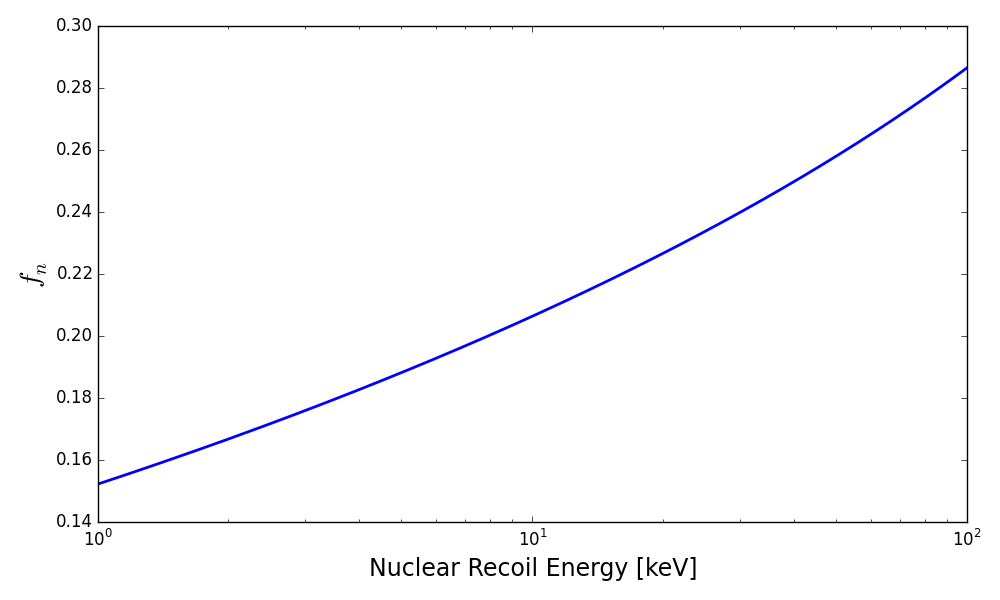
\includegraphics[width=0.8\textwidth]{Lindhard}
\caption{Fraction of nuclear energy passed to atomic motion in xenon using Lindhard's theory (\citeref{Lindhard1965}).}
\label{fig:lindhard}
\end{figure}






In addition to improving the likelihood of spin-independent DM-nucleon scattering (\eqnref{eq:dr_de_final}), the average molar mass
$A = 131.293\ \mathrm{g\ mol^{-1}}$ provides much better stopping power than its noble gas counterparts.  The stopping power $dE/dx$
is the amount of energy lost per distance, and at low energies can be broken down into electronic and nuclear stopping power.

The electronic stopping power is the energy lost due to electronic excitations as a particle travels through the detector.  

The strong self-shielding of xenon grants a larger fiducial volume (FV) - the physical
region of search.

In a dual-phase LXe detector an electric field is applied to measure the freed electrons.  There is a small gap of gas xenon (GXe)
that the $e^{-}$ are pulled towards, at which point they are extracted across, producing proportional, or secondary scintillation.



% for stopping power look at A Model of Nuclear Recoil Scintillation Efficiency in Noble Liquids
%D.-M. Mei a,∗ Z.-B. Yin a,b,1, L.C. Stonehill c, A. Hime c


%Lewin and Smith (1996) - Lindhard factor
%Doke et al., 2002 - LET
%Miller et al., 1968 - drift velocity



%====================================
\section{Electronic Recoils}
\label{sec:er}



\begin{figure}
 \centering
 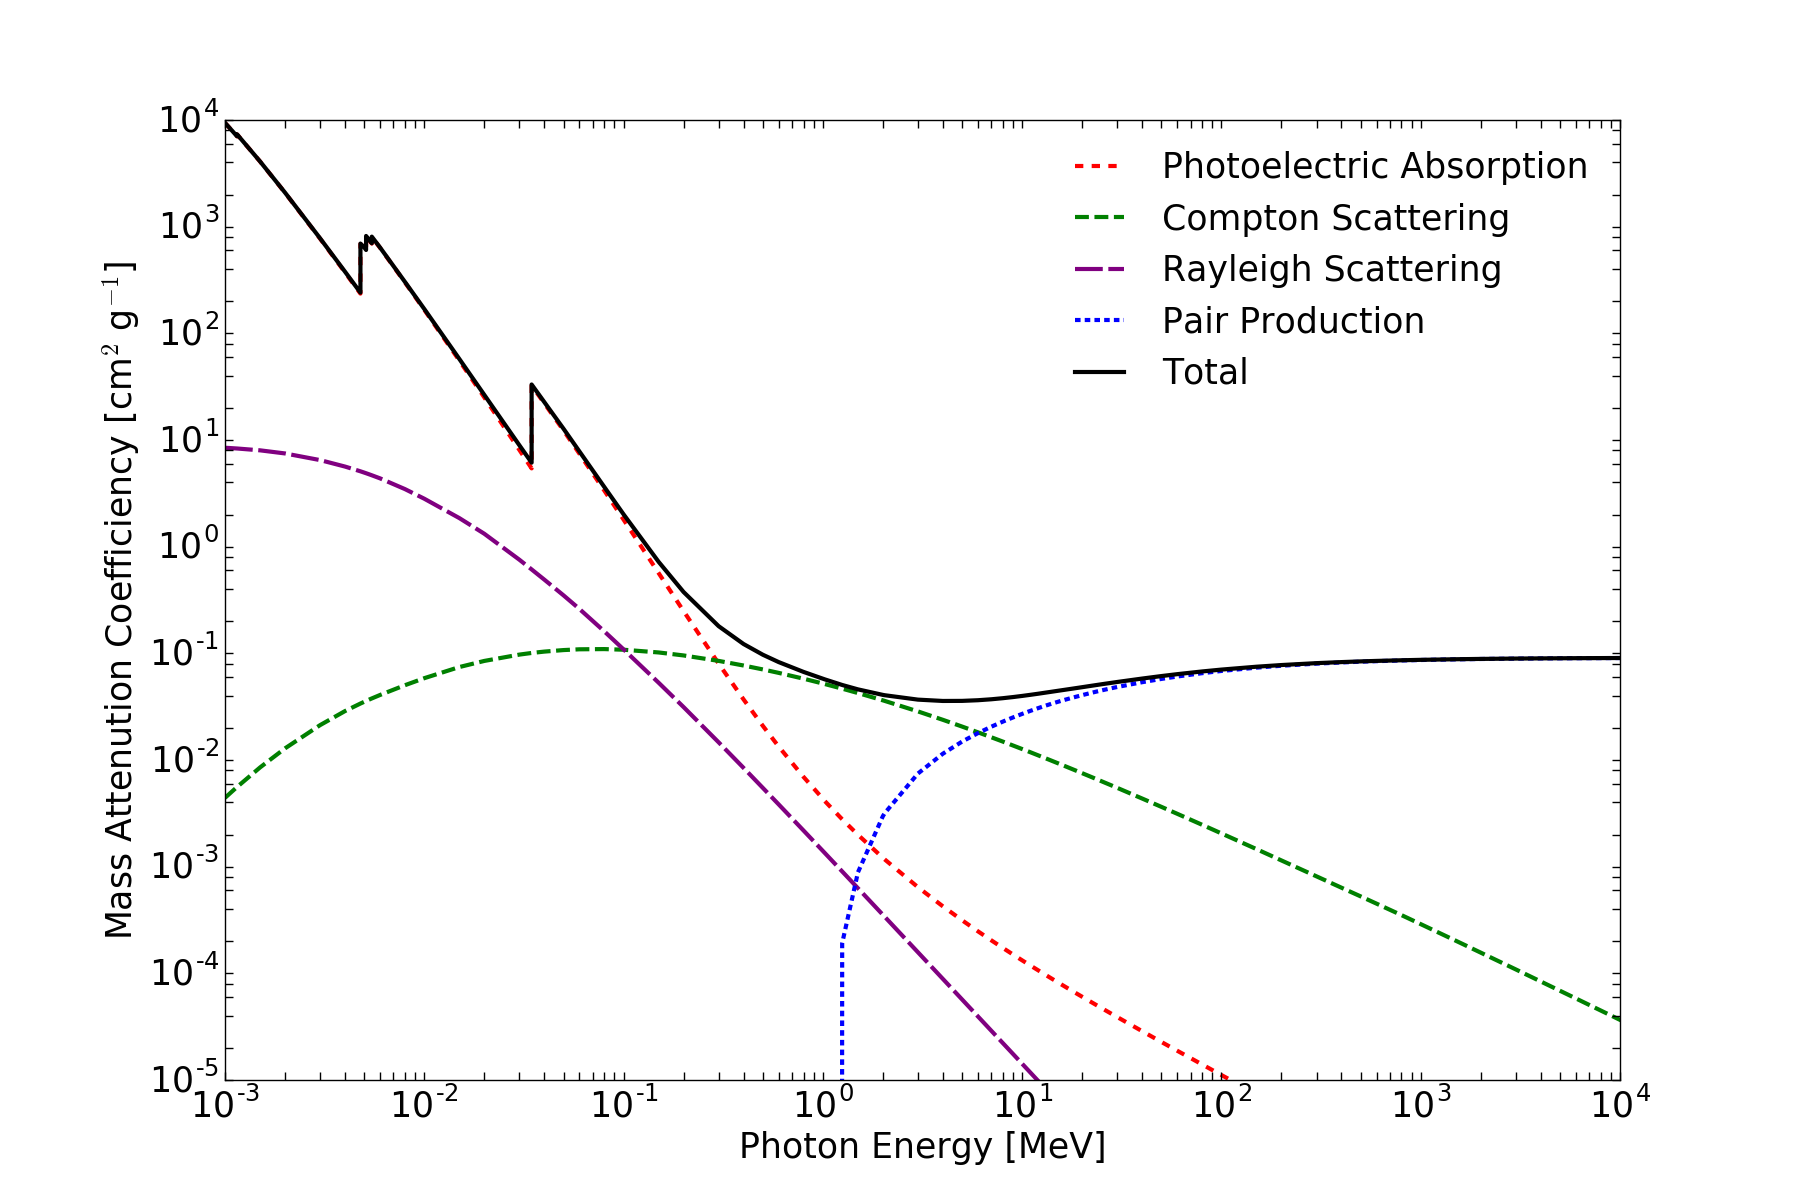
\includegraphics[width=0.8\textwidth]{PhotonAttenuation}
 \label{fig:phot_atten}
\end{figure}


%====================================
\section{Particle Interactions}
\label{sec:particles}



% for kr/xe level
%E Aprile, J Aalbers, F Agostini, M Alfonsi, F. Amaro, M Anthony, F Arneodo, P Barrow, L Baudis, B. Bauermeister, et al., “Removing krypton from xenon by cryogenic distillation to the ppq level,” The European Physical Journal C, vol. 77, no. 5, p. 275, 2017.